% =====================================================================
%  EnergyMind Neighborhood -- Preliminary design: Confidence Scores & Explainability
%  (Challenge Goal 2).  Standalone preview wrapper around a pasteable section.
%
%  TO MERGE INTO THE SHARED REPORT:
%    * copy everything between "BEGIN GOAL 2 SECTION" and "END GOAL 2 SECTION"
%    * copy the bibliography entries at the bottom into the shared bibliography
%    * make sure the shared preamble loads: amsmath, booktabs, tabularx, array,
%      listings, xcolor, tikz (arrows.meta, positioning), enumitem, float,
%      hyperref, and defines the column type L
%    * to use it as a subsection instead, replace \section by \subsection
%      and \subsection by \subsubsection
%
%  Dataset facts quoted below are for node N1 of the EnergyMind dataset (the Phase 1
%  prototype node) and match the Goal 1 report and energymind-tunisia/src/energymind/.
% =====================================================================
\documentclass[11pt,a4paper]{article}
\usepackage[utf8]{inputenc}
\usepackage[T1]{fontenc}
\usepackage[margin=2.5cm]{geometry}
\usepackage{amsmath,amssymb}
\usepackage{booktabs,tabularx,array}
\usepackage{listings}
\usepackage{xcolor}
\usepackage{tikz}
\usetikzlibrary{arrows.meta,positioning}
\usepackage{enumitem}
\usepackage{float}
\usepackage[hidelinks]{hyperref}
\newcolumntype{L}{>{\raggedright\arraybackslash}X}
\lstset{basicstyle=\ttfamily\footnotesize,breaklines=true,frame=single,
        columns=fullflexible,keepspaces=true,backgroundcolor=\color{black!3},
        xleftmargin=2pt,xrightmargin=2pt}

\title{EnergyMind Neighborhood\\[2pt]\large Preliminary Design: Confidence Scores and Explainability}
\author{}
\date{}

\begin{document}
\maketitle

% ===================== BEGIN GOAL 2 SECTION =====================
\providecommand{\GE}{\texttt{GENUINE\_EVENT}}
\providecommand{\MF}{\texttt{METER\_FAULT}}
\providecommand{\SD}{\texttt{SUSPICIOUS\_DATA}}
\providecommand{\ND}{\texttt{NO\_DATA}}
\providecommand{\NORM}{\texttt{NORMAL}}

\section{Goal 2: Confidence Scores and Explainability}
\label{sec:goal2}

\subsection{Goal and Requirements}
The challenge requires that every flagged event comes with a verdict that a human can understand and
verify. The system must output a confidence score, provide a plain-language explanation, and maintain an
auditable decision log that records what was detected, concluded and why. It should use interpretable
approaches and avoid black-box scoring whose reasoning cannot be examined.

Anomalies in this project are equipment and measurement problems, suspected data manipulation (theft or
false data injection) and genuine electrical events. The component therefore chooses among four verdicts,
the same four that the escalation layer of Goal~3 routes: \NORM, \GE{} (the data is right and the grid did
something), \MF{} (a faulty or corrupted meter) and \SD{} (readings that look manipulated). A fifth outcome,
\ND, records a communication loss, which is not scored. The prototype runs on node N1 of the EnergyMind
dataset: one transformer, 30 smart meters on three feeders of 10, readings every 30~minutes.
Table~\ref{tab:requirements} maps each requirement to a design element of this section.

\begin{table}[H]
\centering
\small
\begin{tabularx}{\textwidth}{@{}>{\raggedright\arraybackslash}p{3.4cm}LL@{}}
\toprule
\textbf{Requirement} & \textbf{Design element} & \textbf{Artifact produced} \\
\midrule
Confidence score & Calibrated probability of each of the four verdicts, obtained by multinomial Platt scaling of a few inspectable inputs (Section~\ref{sec:confidence}) & Fields \texttt{class\_probabilities}, \texttt{confidence}, \texttt{band}; calibration curve, Brier score \\ \\
Plain-language explanation & Rules + SHAP $\rightarrow$ evidence $\rightarrow$ RAG $\rightarrow$ LLM text, checked against the rule trace, the SHAP ranking and the logged evidence before it is shown (Section~\ref{sec:language}) & Verdict card; field \texttt{llm\_diagnosis} with the result of the faithfulness check \\ \\
Auditable decision log & One hash-chained record per flagged meter-day (Section~\ref{sec:log}) & \texttt{decision\_log.jsonl} \\ \\
Record what was detected, concluded and why & Three explicit blocks in every record: \texttt{detected}, \texttt{concluded}, \texttt{why} & Rule trace, SHAP evidence, neighborhood support \\ \\
Interpretable approaches & Rule-backed verdicts; SHAP on the detector scores; a calibration model whose coefficients can be printed & No verdict whose reasoning cannot be inspected \\
\bottomrule
\end{tabularx}
\caption{Requirements of Challenge Goal 2 and where this design meets them.}
\label{tab:requirements}
\end{table}

\subsection{Inputs and Outputs of this Component}
\label{sec:io}
The detection layer of Goal~1 works on \emph{meter-days} (48 readings of one meter) and, for every flagged
meter-day, passes on: the stack decision and each detector's score (rules, robust $z$, CUSUM, Isolation
Forest, One-Class SVM, autoencoder); which rules fired, with the measured value and threshold; the
neighborhood support (share of the other 9 meters of the feeder flagged the same day); the state of the
feeder energy-balance alarm; and the autoencoder's per-feature reconstruction error. This component adds a
few evidence quantities computed from the same day's readings (Section~\ref{sec:evidence}) and produces, for
every flagged meter-day, a verdict with its sub-type, the four class probabilities and a confidence band, the
supporting evidence, a plain-language explanation and one decision-log record. The class probabilities are
the input of the Goal~3 escalation layer.

\subsection{Design Principles}
\begin{enumerate}[leftmargin=*,itemsep=2pt]
  \item \textbf{The LLM only describes.} The language model never detects an anomaly and never changes a verdict or a confidence value. This follows the conclusion of the rule-aware prompting work that the main value of an LLM here is a readable rationale for the operator rather than a replacement for the detector~\cite{ruleaware}.
  \item \textbf{Every statement is traceable.} Each statement in an explanation points to a logged item: a rule that fired, a feature value, or a SHAP contribution.
  \item \textbf{Confidence is measured.} The score is calibrated on labeled events and its quality is evaluated like any other output of the system (Section~\ref{sec:evaluation}).
  \item \textbf{No explanation without evidence.} If the generated text fails the faithfulness check, the structured evidence summary is shown instead.
\end{enumerate}

\subsection{Evidence Available to the Explanation Layer}
\label{sec:evidence}
We index a flagged meter-day by meter $i$ and day $t$. Goal~1 supplies the detector scores, the fired rules
and the neighborhood support $s_{i,t}$; the neighborhood-support idea follows prior work that adjusts an
anomaly score using temporal context and the neighborhood~\cite{multiuser}. This component computes the
evidence vector $\mathbf{e}_{i,t}$ of Table~\ref{tab:evidence} from the meter's 48 readings. We write $E$ for
the energy imported in a 30-minute interval ($\Delta t=0.5$~h), $V$, $I$ and $\mathrm{PF}$ for voltage,
current and power factor, $V^{\mathrm{head}}$ for the voltage measured at the head of the feeder and $X$ for
the exported PV energy. Baselines (profiles, medians, scales) are learned on clean meter-days only, i.e.\ days
whose 48 readings are all labelled normal.

\begin{table}[H]
\centering
\small
\begin{tabularx}{\textwidth}{@{}>{\raggedright\arraybackslash}p{1.3cm}>{\raggedright\arraybackslash}p{6.2cm}L@{}}
\toprule
\textbf{Symbol} & \textbf{Definition} & \textbf{What it tells a human} \\
\midrule
$v^{0}_{i,t}$ & Share of readings with $V=0$, or a \texttt{power\_fail} entry in the meter's event log & Supply was lost: the meter is reporting a real outage \\ \\[2pt]
$g_{i,t}$ & Share of missing readings & Communication loss \\ \\[2pt]
$\phi_{i,t}$ & Longest run of readings in which energy \emph{and} voltage are both unchanged (only while $V>0$ and $X=0$) & A stuck meter freezes every channel; real voltage never repeats for hours \\ \\[2pt]
$\rho_{i,t}$ & Median over the day of $E\,/\,(V I\,\mathrm{PF}\,\Delta t/1000)$, using only readings with $V>0$, $X=0$ and an expected energy above 0.02~kWh & Electrical consistency: 1 when energy, voltage and current agree; skipped while the home exports PV \\ \\[2pt]
$s_{i,t}$ & Share of the other 9 meters of the feeder flagged the same day (from Goal~1) & One house, part of the feeder, or the whole feeder \\ \\[2pt]
$\Delta V_{i,t}$ & 24-h median of $V-V^{\mathrm{head}}$ & A meter cannot read more than its feeder head: a positive excess is a voltage-sensor offset \\ \\[2pt]
$\delta_{i,t}$ & Relative drop of the day's energy below the meter's own 28-day profile & How much less than usual this home reports \\ \\[2pt]
$b_{i,t}$ & Feeder energy-balance alarm (from Goal~1): on when the feeder's daily loss has moved away from its seasonal reference & Energy is disappearing (or appearing) somewhere on this feeder \\ \\[2pt]
$\kappa^{\mathrm{tamp}}_{i,t}$ & \texttt{magnetic\_tamper} or \texttt{cover\_open} in the meter's event log & Weak hint of physical tampering (the log also has false alarms) \\ \\[2pt]
$c^{\mathrm{drift}}_{i,t}$ & CUSUM alarm of Goal~1 on the meter's voltage offset, or slope of the meter's share of the feeder over 14 days & Slow drift or a persistent offset \\ \\[2pt]
$\pi_{i,t}$ & Number of consecutive flagged days for this meter while its neighbors are not flagged & How long the deviation has lasted \\
\bottomrule
\end{tabularx}
\caption{Evidence vector $\mathbf{e}_{i,t}$ of a flagged meter-day.}
\label{tab:evidence}
\end{table}

\paragraph{Why these quantities, on this dataset.} Three facts of node N1 shaped the list.
(i) A supply loss is recorded as zeros, not as missing data: in N1 the 684 readings of outages, load
shedding, cable faults and the transformer trip have $V=0$, while only communication losses are blank. Without
$v^{0}$ a flat zero would look like a frozen meter. (ii) The consistency $\rho$ is meaningful because the
dataset's \emph{data-only} injections edit the energy field alone ($\rho\approx0.64$--$0.69$, or $1.68$ for
inflated readings), while honest meters already carry about 1\% measurement error. Without the export gate,
$\rho$ would fire on 39\% of the clean readings of N1's three PV homes; with it, on 0.06\% of all clean
readings. (iii) Sensor bias and physical bypass scale energy \emph{and} current together, so $\rho$ stays at 1
for them; what reveals a bypass is a large drop $\delta$ against the meter's own history together with the
feeder balance $b$.

\subsection{Rule-Backed Verdict Layer}
\label{sec:rules}
The rule-backed scoring turns the evidence vector into a verdict and a sub-type (Figure~\ref{fig:rules}).
Rules are evaluated in a fixed order, so the first matching rule is the one reported, and its identifier
appears in the log and in the explanation. The order follows what makes the other evidence unreliable: a lost
supply first (otherwise a flat zero looks like a frozen meter), then missing and frozen data, then physical
consistency, which separates a manipulated or corrupted value from a real change, and only then the
neighborhood support, which decides between a feeder-wide event and a local one. The split between sudden
problems (R2, R3) and slow ones (R5, R5b) mirrors the split between point and contextual anomalies reported for
smart-meter data~\cite{timefreq}.

\begin{figure}[H]
\centering
\resizebox{\textwidth}{!}{%
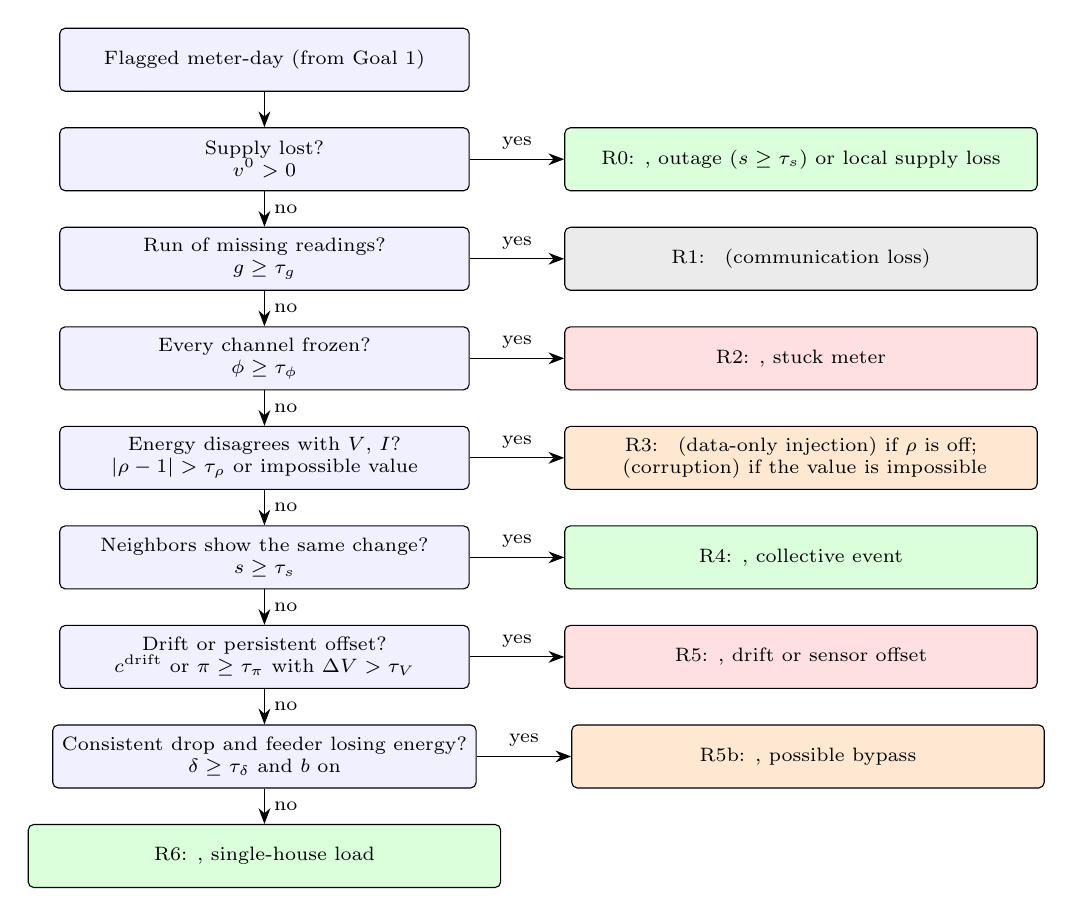
\begin{tikzpicture}[
  node distance=4.5mm and 12mm,
  q/.style={draw,rounded corners=2pt,fill=blue!6,align=center,minimum width=52mm,minimum height=8mm,font=\scriptsize},
  r/.style={draw,rounded corners=2pt,align=center,minimum width=60mm,minimum height=8mm,font=\scriptsize},
  fault/.style={r,fill=red!12}, event/.style={r,fill=green!14}, susp/.style={r,fill=orange!18},
  nodata/.style={r,fill=black!8},
  >={Stealth[length=2mm]}, lab/.style={font=\scriptsize,midway,above}]
\node[q] (s0) {Flagged meter-day (from Goal 1)};
\node[q,below=of s0] (q0) {Supply lost?\\ $v^{0}>0$};
\node[q,below=of q0] (q1) {Run of missing readings?\\ $g\ge\tau_g$};
\node[q,below=of q1] (q2) {Every channel frozen?\\ $\phi\ge\tau_\phi$};
\node[q,below=of q2] (q3) {Energy disagrees with $V$, $I$?\\ $|\rho-1|>\tau_\rho$ or impossible value};
\node[q,below=of q3] (q4) {Neighbors show the same change?\\ $s\ge\tau_s$};
\node[q,below=of q4] (q5) {Drift or persistent offset?\\ $c^{\mathrm{drift}}$ or $\pi\ge\tau_\pi$ with $\Delta V>\tau_V$};
\node[q,below=of q5] (q6) {Consistent drop and feeder losing energy?\\ $\delta\ge\tau_\delta$ and $b$ on};
\node[event,below=of q6] (e2) {R6: \GE{}, single-house load};
\node[event,right=of q0] (r0) {R0: \GE{}, outage ($s\ge\tau_s$) or local supply loss};
\node[nodata,right=of q1] (r1) {R1: \ND{} (communication loss)};
\node[fault,right=of q2] (r2) {R2: \MF{}, stuck meter};
\node[susp,right=of q3] (r3) {R3: \SD{} (data-only injection) if $\rho$ is off;\\ \MF{} (corruption) if the value is impossible};
\node[event,right=of q4] (r4) {R4: \GE{}, collective event};
\node[fault,right=of q5] (r5) {R5: \MF{}, drift or sensor offset};
\node[susp,right=of q6] (r5b) {R5b: \SD{}, possible bypass};
\draw[->] (s0)--(q0);
\foreach \a/\b in {q0/q1,q1/q2,q2/q3,q3/q4,q4/q5,q5/q6,q6/e2}{\draw[->] (\a)--node[right,font=\scriptsize]{no}(\b);}
\foreach \a/\b in {q0/r0,q1/r1,q2/r2,q3/r3,q4/r4,q5/r5,q6/r5b}{\draw[->] (\a)--node[lab]{yes}(\b);}
\end{tikzpicture}}
\caption{Rule cascade turning the evidence vector into a verdict. All thresholds $\tau$ are fitted by
event-grouped cross-validation (Section~\ref{sec:confidence}) and stored in a versioned configuration file
(\texttt{configs/thresholds.yaml}), not hard-coded.}
\label{fig:rules}
\end{figure}

\begin{table}[H]
\centering
\small
\begin{tabularx}{\textwidth}{@{}>{\raggedright\arraybackslash}p{0.9cm}>{\raggedright\arraybackslash}p{3.7cm}>{\raggedright\arraybackslash}p{3.1cm}L@{}}
\toprule
\textbf{Rule} & \textbf{Condition} & \textbf{Verdict} & \textbf{Reason sentence (template)} \\
\midrule
R0 & $v^{0}>0$ & \GE{} (outage if $s\ge\tau_s$; local supply loss if 2--6 meters; single meter otherwise) & ``Voltage was 0~V on \{n\} of \{N\} meters of feeder \{f\} for \{hours\} h: supply was lost and the meter is reporting correctly.'' \\ \\
R1 & $g\ge\tau_g$ & \ND{} (communication loss) & ``\{share\} of this meter's readings did not arrive; no verdict is possible for this period.'' \\ \\
R2 & $\phi\ge\tau_\phi$ & \MF{} (stuck meter) & ``Energy and voltage have not changed for \{hours\} h; real voltage always varies.'' \\ \\
R3 & $|\rho-1|>\tau_\rho$ & \SD{} (data-only injection); \MF{} (corruption) if $E<0$, $E=99.999$ or $\times1000$ & ``Reported energy is \{ratio\}$\times$ what voltage and current imply (limit \{tau\}); voltage and current look normal.'' \\ \\
R4 & $s\ge\tau_s$, $\rho$ consistent & \GE{} (collective) & ``\{n\} of \{N\} meters on feeder \{f\} changed together and their electrical readings agree.'' \\ \\
R5 & $s<\tau_s$, $c^{\mathrm{drift}}$ on, or $\Delta V>\tau_V$ for $\ge\tau_\pi$ days & \MF{} (drift or sensor offset) & ``This meter reads \{dv\}~V above its feeder head, which is physically impossible, for \{days\} days.'' \\ \\
R5b & $s<\tau_s$, $\rho$ consistent, $\delta\ge\tau_\delta$, $b$ on & \SD{} (possible bypass) & ``This home reports \{pct\}\% less than its usual level for \{days\} days while feeder \{f\} loses \{gap\}\% more energy than usual; voltage and current agree with the reported energy, which fits a physical bypass.'' \\ \\
R6 & $s<\tau_s$, $\rho$ consistent, short-lived & \GE{} (single-house load) & ``Only this home changed, briefly, and energy, voltage and current agree: an appliance switching on is the likely cause.'' \\
\bottomrule
\end{tabularx}
\caption{Rule table. The tamper flag $\kappa^{\mathrm{tamp}}$ is reported as supporting evidence for R5b but
never decides a verdict: in N1 it appears on 4 falsified readings and on 55 clean ones.}
\label{tab:rules}
\end{table}

\paragraph{Notes on the rules.}
\begin{itemize}[leftmargin=*,itemsep=2pt]
  \item \textbf{R0 before R2.} Without it, every outage, load-shedding period, cable fault and transformer trip
        of N1 would be reported as a stuck meter, the opposite of the right answer.
  \item \textbf{R3 before R4.} A coordinated injection hits three meters of one feeder, so it could pass the
        neighborhood test; its energy disagrees with $V$ and $I$, so R3 catches it first.
  \item \textbf{Suspect channel.} For R3 the suspect channel is energy by construction. For the other
        verdicts it is the feature with the largest autoencoder reconstruction error passed on by Goal~1; for
        faults that scale every channel (bias, bypass, frozen meter, clock shift) no single channel is
        named.
  \item \textbf{R5b before R6.} An isolated, electrically consistent drop is not automatically an appliance:
        when it lasts and the feeder starts losing energy at the same time, a bypass is the better
        explanation. A short, isolated, consistent change with no balance alarm stays a single-house load.
  \item \textbf{What the rules cannot settle.} Goal~1 found that small sensor biases and gain drifts are
        rarely flagged at all, and that the balance alarm names a feeder, not a meter. When $b$ is on but no
        meter shows a clear drop, the case is logged as \SD{} with a low confidence band, which sends it to
        a human (Goal~3).
\end{itemize}

\subsection{Confidence Score}
\label{sec:confidence}
For each flagged meter-day the component outputs a probability for each of the four verdicts,
$p_{i,t}(c)$ for $c\in\{\NORM,\GE,\MF,\SD\}$. The confidence of the reported verdict is
$c_{i,t}=p_{i,t}(\hat c)$, and the full vector is passed to Goal~3, which needs the margin between the two most
likely verdicts and the set of plausible alternatives. The probabilities are built from three inputs, each
of which can be inspected on its own:
\begin{enumerate}[leftmargin=*,itemsep=2pt]
  \item the Goal~1 stack score $\tilde a_{i,t}$: the largest detector score, each standardized against its
        distribution on clean meter-days;
  \item the \emph{rule margin} $m_{i,t}\in[0,1]$, which measures how clearly the rule that fired was
      satisfied. Each condition of that rule compares an evidence value $e_j$ with a threshold $\tau_j$.
      For each condition we compute its relative distance from the threshold,
      $\min\{1,\,|e_j-\tau_j|/\tau_j\}$, which is $0$ when the value sits exactly on the threshold and
      $1$ when it is at least one threshold-width away. The margin $m_{i,t}$ is the smallest of these
      values over the conditions of the rule, so a verdict is only as clear as its most borderline
      condition;
  \item the \emph{detector agreement} $\kappa_{i,t}\in\{0,\dots,6\}$: how many of the six Goal~1 detectors
        flagged the day, in the spirit of the explicit sigma rule used in rule-aware
        prompting~\cite{ruleaware}.
\end{enumerate}
Together with a one-hot code of the rule that fired, these inputs are mapped to probabilities by multinomial
Platt scaling, one of the calibration techniques listed in the trust-calibration literature~\cite{trustcal}:
a multinomial logistic regression whose coefficients can be printed and read,
\begin{equation}
  p_{i,t}(c)\;=\;\frac{\exp\bigl(\beta_{c,0}+\beta_{c,1}\tilde a_{i,t}+\beta_{c,2}m_{i,t}+\beta_{c,3}\kappa_{i,t}+\gamma_{c,r(i,t)}\bigr)}
  {\sum_{c'}\exp\bigl(\beta_{c',0}+\beta_{c',1}\tilde a_{i,t}+\beta_{c',2}m_{i,t}+\beta_{c',3}\kappa_{i,t}+\gamma_{c',r(i,t)}\bigr)},
\end{equation}
where $r(i,t)$ is the rule that fired. The target is the true class of the meter-day, known from the dataset
labels. If the calibration curve is poor, isotonic regression, another technique from the same
literature~\cite{trustcal}, is the alternative.

\paragraph{Confidence band.} The probability is shown to operators as a band: HIGH above 0.90, LOW below
0.60, MEDIUM in between (Goal~3 thresholds). A class's band may be HIGH only if its calibration has been
validated on at least 30 out-of-fold events. In N1 this holds for \GE{} (37 events) and \MF{} (33), not for
\SD{} (8 events, one per manipulation type), so \SD{} verdicts are capped at MEDIUM and are always reviewed by
a human.

We do not assume that the result is calibrated; we measure it (Section~\ref{sec:evaluation}). This matters because the confidence-based routing of Goal~3 assumes reasonably calibrated confidence: an overconfident model may delegate dangerous decisions to the AI, and an underconfident one may defer everything to humans~\cite{trustcal}.

\paragraph{Data used for fitting.} A split by calendar period does not work on this dataset: in N1,
November--December contain no falsification and no sensor-bias event, and September--October only two
falsifications. Baselines (profiles, medians, scales) therefore use clean meter-days only, and the thresholds
$\tau$ and the coefficients $\beta,\gamma$ are fitted by 5-fold cross-validation over the whole year, with folds
grouped by event (\texttt{gt\_event\_id}), so that no event is split between fitting and testing; within each
training fold, $\tau$ is fitted on one half of the events and $\beta,\gamma$ on the other. Clean days are
assigned to folds in meter-week blocks to keep near-duplicate neighboring readings from leaking between sets.
All reported numbers are out-of-fold, per event, with Wilson 95\% intervals.

\subsection{From Evidence to Plain Language}
\label{sec:language}
Figure~\ref{fig:pipeline} shows how the verdict and the evidence become the text that the operator reads,
following the chain rules and SHAP $\rightarrow$ evidence $\rightarrow$ RAG $\rightarrow$ LLM text. Full
explanations are generated only for flagged meter-days, never for every normal reading, to keep latency and
cost down.

\begin{figure}[htbp]
\centering
\resizebox{\textwidth}{!}{%
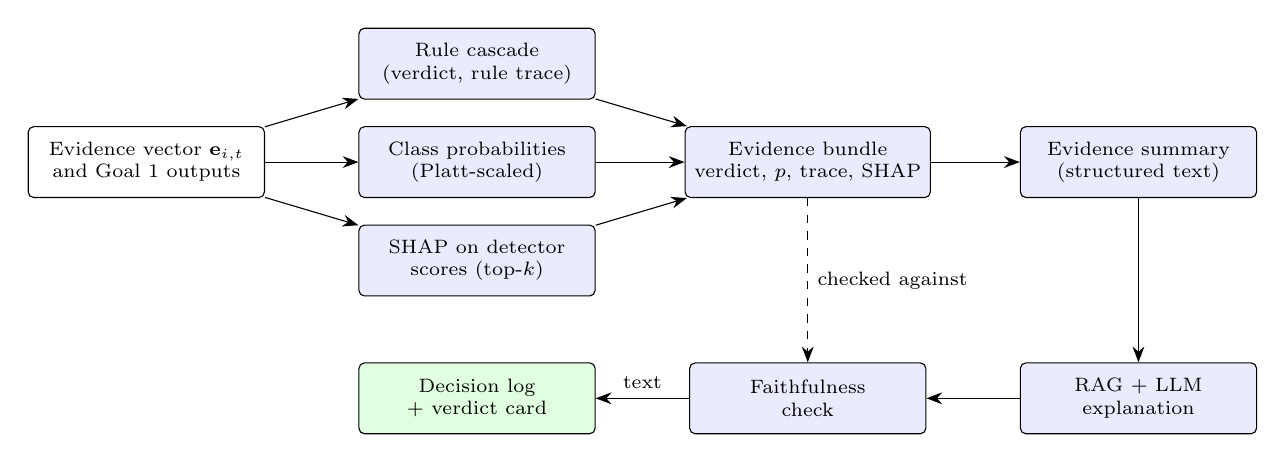
\begin{tikzpicture}[
  b/.style={draw,rounded corners=2pt,align=center,minimum width=30mm,minimum height=9mm,font=\scriptsize},
  core/.style={b,fill=blue!8}, result/.style={b,fill=green!12},
  >={Stealth[length=2mm]}]
\node[b] (ev) at (0,0) {Evidence vector $\mathbf{e}_{i,t}$\\ and Goal 1 outputs};
\node[core] (rules) at (4.2,1.25) {Rule cascade\\ (verdict, rule trace)};
\node[core] (cal) at (4.2,0) {Class probabilities\\ (Platt-scaled)};
\node[core] (shap) at (4.2,-1.25) {SHAP on detector\\ scores (top-$k$)};
\node[core] (bundle) at (8.4,0) {Evidence bundle\\ verdict, $p$, trace, SHAP};
\node[core] (tpl) at (12.6,0) {Evidence summary\\ (structured text)};
\node[core] (llm) at (12.6,-3.0) {RAG + LLM\\ explanation};
\node[core] (val) at (8.4,-3.0) {Faithfulness\\ check};
\node[result] (log) at (4.2,-3.0) {Decision log\\ + verdict card};
\draw[->] (ev)--(rules); \draw[->] (ev)--(cal); \draw[->] (ev)--(shap);
\draw[->] (rules)--(bundle); \draw[->] (cal)--(bundle); \draw[->] (shap)--(bundle);
\draw[->] (bundle)--(tpl);
\draw[->] (tpl)--(llm);
\draw[->] (llm)--(val);
\draw[->,dashed] (bundle)--node[right,font=\scriptsize]{checked against}(val);
\draw[->] (val)--node[above,font=\scriptsize]{text}(log);
\end{tikzpicture}}
\caption{Explanation pipeline.}
\label{fig:pipeline}
\end{figure}

The language model only receives the evidence bundle and retrieved snippets and writes about them; the faithfulness check compares its text with the same bundle. If the check rejects the text, the evidence summary is logged and shown instead.

\subsubsection*{Step 1: attributions with SHAP}
The rules say what kind of problem it is; SHAP says why the detectors flagged the meter-day in the first
place. SHAP assigns each input feature a value showing how much it pushed a detector's score for this day up
or down relative to a baseline, and it is model-agnostic. We apply the \texttt{shap} library to the Isolation
Forest and the autoencoder of Goal~1, on their daily features, and only on flagged meter-days. Each feature
is tied to a sentence template by a small lexicon, which is how a number becomes a statement
(Table~\ref{tab:lexicon}).

\begin{table}[H]
\centering
\small
\begin{tabularx}{\textwidth}{@{}>{\raggedright\arraybackslash}p{3.6cm}L@{}}
\toprule
\textbf{Goal 1 feature} & \textbf{Sentence template} \\
\midrule
Profile residual & ``Today this home used \{x\} kWh against a usual \{y\} kWh for this season and day type.'' \\ \\
Share of the feeder & ``This home's share of feeder \{f\} has moved by \{pct\}\% compared with the last four weeks.'' \\ \\
Physics ratio & ``Reported energy is \{ratio\}$\times$ what voltage and current imply.'' \\ \\
$V$ minus feeder-head $V$ & ``This meter reads \{dv\}~V \{above/below\} the head of its feeder; usually \{dv0\}~V.'' \\ \\
Longest frozen run & ``Energy and voltage stayed identical for \{hours\} h.'' \\ \\
Lag gain against profile & ``Today's pattern matches the usual one best when shifted by \{h\} h (clock problem?).'' \\ \\
Similarity to last week & ``Today's readings are almost identical to the same day last week (possible replay).'' \\
\bottomrule
\end{tabularx}
\caption{Excerpt of the feature lexicon that turns attributions into sentences (one entry per Goal~1
feature; the evidence quantities of Table~\ref{tab:evidence} have their own sentences in
Table~\ref{tab:rules}).}
\label{tab:lexicon}
\end{table}

\subsubsection*{Step 2: structured evidence summary}
A deterministic step assembles the evidence bundle into a summary: a headline (verdict, channel, confidence
and band), the strongest reasons (the rule's reason sentence first, then the highest SHAP contributions), the
runner-up verdict, a \emph{what would change this verdict} line generated from the rule thresholds, and a
suggested check. This follows the recommendation, in a review of AI approaches for smart-grid reliability, to
combine local feature attribution, counterfactuals and logged explanations~\cite{review2025}. The summary is the
input of the language model and also the text shown if the faithfulness check fails. An illustrative card
(modelled on the data-only injection of feeder N1-F3 in May; values for illustration):

\begin{lstlisting}
Event N1-2025-05-03-M026 | Meter N1-M026 (feeder N1-F3) | 2025-05-03
VERDICT: SUSPICIOUS DATA, energy channel     CONFIDENCE: 0.74 (MEDIUM)
Runner-up: METER FAULT (0.19)

Why:
 1. Reported energy is 0.65x what voltage and current imply
    (limit +/-5%) -> rule R3.
 2. Isolated: 0 of 9 other meters on feeder N1-F3 changed.
 3. Voltage and current follow this home's usual pattern; only the
    energy field is low.

This would be a METER FAULT instead if: the value were impossible
(negative, x1000, 99.999); a GENUINE EVENT if >= 3 neighbors changed
the same way and energy matched voltage and current.

Suggested check: read the meter register on site and compare it with
the reported energy; inspect the data path (gateway, head-end).
\end{lstlisting}

\subsubsection*{Step 3: RAG and LLM explanation with a faithfulness check}
The language model turns the evidence summary into a readable diagnosis and can add context that a
template cannot, such as earlier incidents at the same meter. It receives the evidence bundle as structured
data together with a few retrieved snippets from a small corpus: descriptions of the fault kinds, the
anomaly taxonomy and earlier log entries for the same meter. It is asked to justify the verdict against an
explicit, stated rule, as in rule-aware prompting for grid telemetry~\cite{ruleaware}, and it may not alter
the verdict or the confidence.

Before the text is displayed, a faithfulness check compares it with the evidence bundle:
\begin{itemize}[leftmargin=*,itemsep=1pt]
  \item every reason it names must be a fired rule or one of the top-$k$ SHAP features;
  \item every number it quotes must match the logged value up to rounding;
  \item the verdict, the confidence and the band must be those in the log.
\end{itemize}
If any test fails, the evidence summary is shown instead and the event is logged with that fact. The check
is needed because a study of retrieval-augmented LLM post-processing for anomaly detection found only a
modest gain from the language model, and explanation faithfulness did not improve with retrieval~\cite{ragaudit}.
We therefore treat the LLM as a layer that describes the evidence, not as a source of reasoning.

\subsection{Auditable Decision Log}
\label{sec:log}
Every flagged meter-day produces one record in an append-only JSON Lines file. Each record stores the hash of
the previous one, so a later edit or deletion breaks the chain. The record is grouped around the three
questions the challenge asks (Table~\ref{tab:log}); an abridged example follows. The escalation layer of
Goal~3 appends its own \texttt{governance} block (route, rules fired, operator judgement, final decision) to the
same record; this section defines only the fields produced by detection, conclusion and explanation. The full
schema is \texttt{docs/decision\_log\_schema.json} in the project repository.

\begin{table}[H]
\centering
\small
\begin{tabularx}{\textwidth}{@{}>{\raggedright\arraybackslash}p{2.8cm}L@{}}
\toprule
\textbf{Block} & \textbf{Fields} \\
\midrule
\texttt{detected} & event id, day, node, feeder and meter id, model version, stack score, per-detector scores, per-feature reconstruction error, flag \\ \\
\texttt{concluded} & verdict, sub-type, suspect channel, class probabilities, confidence, band \\ \\
\texttt{why} & rule trace (rule id, measured value, threshold, passed or not), SHAP evidence, neighborhood support, feeder-balance alarm, threshold version, retrieved sources \\ \\
\texttt{explanation} & LLM diagnosis, result of the faithfulness check, text actually shown \\ \\
\texttt{ground\_truth} & filled afterwards, for evaluation only: dataset label, sub-type, event id \\
\bottomrule
\end{tabularx}
\caption{Structure of a decision log record.}
\label{tab:log}
\end{table}

\begin{lstlisting}
{"event_id":"N1-2025-05-03-M026","ts":"2025-05-03","node_id":"N1",
 "feeder_id":"N1-F3","meter_id":"N1-M026",
 "detected":{"model_version":"detect-0.1","fused_score":4.8,"flag":true,
   "detector_scores":{"rules":1,"robust_z":9.1,"svm":2.3,"ae":6.4}},
 "concluded":{"verdict":"SUSPICIOUS_DATA","subtype":"data_only_injection",
   "suspect_channel":"energy","confidence":0.74,"band":"MEDIUM",
   "class_probabilities":{"NORMAL":0.02,"GENUINE_EVENT":0.05,
                          "METER_FAULT":0.19,"SUSPICIOUS_DATA":0.74}},
 "why":{"rules":[{"id":"R3","measured":0.65,"threshold":0.05,"passed":true},
                 {"id":"R4","measured":0.0,"threshold":0.3,"passed":false}],
        "shap":[["physics_ratio",0.52],["profile_residual",0.21]],
        "neighbour_support":"0/9","balance_alarm":false,
        "thresholds_version":"0.1-phase1"},
 "explanation":{"llm_diagnosis":"...","faithfulness":"pass","shown":"llm"},
 "prev_hash":"9f2c...","hash":"41ab..."}
\end{lstlisting}
(The values are invented for illustration.) The record keeps the exact inputs and the version of the
thresholds and models, so a verdict can be reproduced and reviewed later.

\subsection{How We Will Evaluate Explanations and Confidence}
\label{sec:evaluation}
The dataset labels every reading with its class, its exact sub-type and the event it belongs to, so verdicts
and explanations can be tested against ground truth rather than only judged by eye. In N1 the flagged
material comes from 98 events: 37 genuine events, 33 meter faults (25 of them data corruption), 8
falsifications and 20 communication losses. Most manipulation and sensor-fault types occur once, so results are
reported per event, with intervals, and never as a single accuracy figure; we use precision, recall and
false-positive rate per class.

\begin{table}[H]
\centering
\small
\begin{tabularx}{\textwidth}{@{}>{\raggedright\arraybackslash}p{3.1cm}LL@{}}
\toprule
\textbf{Aspect} & \textbf{Measure} & \textbf{Method} \\
\midrule
Confidence quality & Calibration curve and Brier score~\cite{trustcalpage}; verdict accuracy within each band & Out-of-fold, per class and overall \\ \\
Verdict correctness & Precision, recall and false-positive rate per class, with event counts & Against the dataset labels, out-of-fold; also on the \emph{subtle set} \\ \\
Explanation correctness & Share of verdicts whose named channel is the true one (Table~\ref{tab:channels}); share whose scope (isolated, part of the feeder, whole feeder) is right & Labels versus the \texttt{why} block \\ \\
LLM faithfulness & Share of LLM texts accepted by the faithfulness check; kinds of statements rejected & Automatic check on all flagged meter-days \\ \\
Does the LLM help & LLM text versus the plain evidence summary, rated on clarity and correctness (1--5) by several team members who do not know which is which & Sample of flagged meter-days \\ \\
Response latency & Median and 95th-percentile time of rules, SHAP and LLM per flagged meter-day & Timer on the evaluation run \\
\bottomrule
\end{tabularx}
\caption{Evaluation plan for confidence scores and explanations.}
\label{tab:evalplan}
\end{table}

\begin{table}[H]
\centering
\small
\begin{tabularx}{\textwidth}{@{}>{\raggedright\arraybackslash}p{2.4cm}L@{}}
\toprule
\textbf{True channel} & \textbf{Dataset sub-types} \\
\midrule
Energy & \texttt{fdi\_scale}, \texttt{fdi\_evasion}, \texttt{fdi\_inflate}, \texttt{fdi\_replay}, \texttt{coordinated\_fdi}, all data corruption (\texttt{spike\_gain}, \texttt{negative\_value}, \texttt{saturation}, \texttt{unit\_error\_x1000}) \\ \\
Voltage & \texttt{voltage\_offset\_drift} \\ \\
All channels & \texttt{bias\_step}, \texttt{gain\_drift}, \texttt{stuck\_value}, \texttt{clock\_shift}, \texttt{partial\_reduction\_bypass}, \texttt{selective\_bypass}, \texttt{meter\_zeroing}: only the verdict and the scope are scored \\
\bottomrule
\end{tabularx}
\caption{The dataset has no ``injected channel'' column; this fixed mapping from sub-type to channel is used to
score the suspect channel named in the explanation.}
\label{tab:channels}
\end{table}

The \emph{subtle set} is built from existing events, without changing the dataset: the first seven days of
the two gain drifts and of the bias step, and the evasion attack, whose scaling factor wanders to mimic
natural variation.

\subsection{Risks and Limitations}
\label{sec:risks}
\begin{itemize}[leftmargin=*,itemsep=2pt]
  \item \textbf{Few events per type.} Most manipulation and sensor-fault types occur once in N1, so
        per-type results are case studies, not rates; the \SD{} band is capped at MEDIUM for that reason.
  \item \textbf{Simulated data.} Thresholds and calibration coefficients are fitted on one generator's
        anomalies and may be optimistic; results on the subtle set are reported alongside.
  \item \textbf{Physically consistent manipulation.} Bypasses keep energy, voltage and current consistent;
        R5b depends on the feeder-balance alarm of Goal~1, which names a feeder and reacts after 1--2 weeks. A
        meter that under-reports slightly may never reach R5b.
  \item \textbf{PV homes.} The consistency check is skipped while a home exports, so an injection limited to
        export hours would be missed by R3.
  \item \textbf{Weak tamper log.} Tamper codes also appear on clean readings; they support but never decide
        a verdict.
  \item \textbf{Correlated features.} SHAP can spread credit among correlated features. The rule trace is
        therefore the primary explanation and SHAP the supporting one.
  \item \textbf{Cost of SHAP.} SHAP is run only on flagged meter-days and its latency is measured; the rule
        trace remains available if it is too slow.
  \item \textbf{Calibration can drift} across seasons or meters; the calibration curve is checked again on
        later events.
  \item \textbf{Convincing but wrong.} A fluent explanation can raise trust beyond what the evidence
        justifies, so every card shows the confidence band, the runner-up verdict and the counterfactual line.
  \item \textbf{Language model errors.} The faithfulness check and the fallback to the evidence summary
        limit this, and the acceptance rate of the check is reported.
\end{itemize}

% ===================== END GOAL 2 SECTION =======================

\begin{thebibliography}{99}
\bibitem{ruleaware} ``A Rule-Aware Prompt Framework for Structured Numeric Reasoning in Smart Grids,'' arXiv:2512.12794.
\bibitem{ragaudit} ``Component-Level Contributions of Retrieval-Augmented LLM Post-Processing in Streaming Anomaly Detection,'' \emph{Sensors}, 2026.
\bibitem{trustcal} ``Confidence-Based Trust Calibration in Human-AI Teams,'' SAI, vol.~16, no.~12.
\bibitem{trustcalpage} ``Trust Calibration in AI,'' Emergent Mind overview page, \url{https://www.emergentmind.com/topics/trust-calibration-in-ai}.
\bibitem{review2025} ``Comprehensive review of AI-driven approaches for smart grid stability and reliability,'' ScienceDirect, 2025.
\bibitem{timefreq} ``Time and Frequency Domain-based Anomaly Detection in Smart Meter Data,'' arXiv:2504.18231.
\bibitem{multiuser} ``Multi-User Energy Consumption Monitoring and Anomaly Detection with Partial Context Information.''
\end{thebibliography}
\end{document}
